% Synchronous vs asynchronous RL: who waits for whom. Durations are illustrative.
\documentclass[border=8pt]{standalone}
% Shared TikZ style for every figure in "Post-training LLMs with RL" (see ../STYLE.md).
% Visual grammar follows the FME office-hours house style; the one accent colour is fern green.
% Compile with XeLaTeX, two passes (annotated equations remember node positions).
\usepackage{fontspec}
\setmainfont{Avenir Next}[BoldFont={Avenir Next Demi Bold}, ItalicFont={Avenir Next Italic}]
\setsansfont{Avenir Next}[BoldFont={Avenir Next Demi Bold}, ItalicFont={Avenir Next Italic}]
\renewcommand{\familydefault}{\sfdefault}
\hyphenpenalty=10000 \exhyphenpenalty=10000 % no hyphenation in notes and labels
\usepackage{amsmath,amssymb}
\usepackage{tikz}
\usetikzlibrary{arrows.meta,positioning,calc,fit,backgrounds,shapes.geometric,decorations.pathreplacing}

% ---------------- palette ----------------
\definecolor{ink}{HTML}{111111}
\definecolor{grey700}{HTML}{4A4F55}
\definecolor{grey500}{HTML}{6B7178}
\definecolor{grey400}{HTML}{8A9097}
\definecolor{grey300}{HTML}{D5D9DD}
\definecolor{grey100}{HTML}{F4F5F6}
\definecolor{fern}{HTML}{4F7942}       % the one accent: what the figure is about
\definecolor{ferndark}{HTML}{2F4A28}
\definecolor{fernlight}{HTML}{B5CFA8}
\definecolor{ferntint}{HTML}{EAF1E6}
% aliases used by older figure files
\colorlet{gray7}{grey700}\colorlet{gray5}{grey500}\colorlet{gray3}{grey300}\colorlet{gray1}{grey100}

% ---------------- visual grammar ----------------
\tikzset{
  every picture/.style={line cap=round, line join=round, color=ink},
  tensor/.style={draw=ink, line width=0.8pt, fill=white},
  param/.style={draw=grey700, line width=0.8pt, fill=grey100},
  op/.style={draw=grey500, line width=0.8pt, rounded corners=3pt, fill=white, inner sep=4pt, font=\small},
  accent/.style={draw=fern, line width=1.2pt},
  flow/.style={-{Stealth[length=5pt]}, line width=0.8pt, draw=grey700},
  flowa/.style={flow, draw=fern},
  tname/.style={font=\normalsize, text=ink},
  dims/.style={font=\footnotesize, text=grey500},
  note/.style={font=\footnotesize, text=grey700, align=left},
  accentnote/.style={font=\footnotesize, text=fern, align=left},
  lead/.style={draw=grey400, line width=0.5pt},
  stream/.style={draw=grey300, line width=5pt},
  block/.style={draw=grey500, line width=0.8pt, rounded corners=4pt, fill=white, align=center, font=\small, minimum height=0.8cm},
  blocka/.style={block, accent, fill=ferntint},
  frozen/.style={block, fill=grey100},
  plus/.style={circle, draw=grey700, line width=0.8pt, fill=white, inner sep=0pt, minimum size=0.42cm, font=\small},
  junction/.style={circle, fill=grey700, inner sep=0pt, minimum size=4pt},
  wire/.style={line width=0.8pt, draw=grey700},
}

% ---------------- numbered annotation system ----------------
%   markers on the drawing:  \mk{(x,y)}{1}   \mka{(x,y)}{2} (accent)
%   notes column:            \notesat{(x,y)}{width}  then  \note{1}{text}  /  \notea{2}{text}
%   symbols strip:           \symbols{$x$ & prompt \\ $y$ & response}
\tikzset{
  marker/.style={circle, fill=grey700, text=white, font=\footnotesize\bfseries, inner sep=0pt, minimum size=0.46cm},
  markera/.style={marker, fill=fern},
}
\newcommand{\mk}[2]{\node[marker] at #1 {#2}}
\newcommand{\mka}[2]{\node[markera] at #1 {#2}}
\newlength{\notewidth}
\newcommand{\notesat}[2]{%
  \node[inner sep=0pt, minimum size=0pt, anchor=north west] (note0) at #1 {};
  \setlength{\notewidth}{#2}\xdef\lastnote{note0}}
\newcommand{\note}[2]{%
  \node[font=\small, text=ink, align=left, text width=\notewidth, anchor=north west, inner sep=0pt] (note#1) at ($(\lastnote.south west)+(0.55cm,-0.32cm)$) {#2};
  \node[marker] at ($(note#1.north west)+(-0.30cm,-0.15cm)$) {#1};
  \path (note#1.south west) ++(-0.55cm,0) node[inner sep=0pt, minimum size=0pt] (note#1base) {};
  \xdef\lastnote{note#1base}}
\newcommand{\notea}[2]{%
  \node[font=\small, text=ferndark, align=left, text width=\notewidth, anchor=north west, inner sep=0pt] (note#1) at ($(\lastnote.south west)+(0.55cm,-0.32cm)$) {#2};
  \node[markera] at ($(note#1.north west)+(-0.30cm,-0.15cm)$) {#1};
  \path (note#1.south west) ++(-0.55cm,0) node[inner sep=0pt, minimum size=0pt] (note#1base) {};
  \xdef\lastnote{note#1base}}
\newcommand{\symbols}[1]{%
  \node[anchor=north west, inner sep=0pt, align=left, font=\small, text=grey700] (symbols)
    at ($(\lastnote.south west)+(0,-0.75cm)$)
    {\textcolor{grey400}{\scriptsize\bfseries SYMBOLS}\\[3pt]
     \begin{tabular}{@{}l@{\hspace{8pt}}l@{}}#1\end{tabular}};
  \draw[grey300, line width=0.5pt] ($(symbols.north west)+(0,0.18cm)$) -- ++(\notewidth+0.55cm,0);}

% ---------------- glyphs ----------------
\tikzset{
  expand/.style={draw=grey700, line width=0.8pt, fill=grey100, trapezium, trapezium stretches body,
                 trapezium left angle=64, trapezium right angle=64, shape border rotate=180,
                 minimum height=0.72cm, align=center, font=\small, inner xsep=2pt},
  contract/.style={expand, shape border rotate=0},
  silubox/.style={block, path picture={
      \begin{scope}[sharp corners, shift={($(path picture bounding box.west)+(0.45,-0.05)$)}, x=0.1cm, y=0.1cm]
        \draw[grey300, line width=0.4pt] (-3,0) -- (2.6,0);
        \draw[grey500, line width=1pt, domain=-3:2.4, samples=30] plot (\x, {\x/(1+exp(-\x))});
      \end{scope}}},
}

% ---------------- annotated equations (arrow + plain-language label per term) ----------------
% \tm{name}{math}: wrap one term of a formula in a named node. Put the formula node at (0,0)
% with anchor=base west, otherwise the remembered positions are offset.
\newcommand{\tm}[2]{\tikz[remember picture,baseline=(#1.base)]{\node[inner sep=1pt,outer sep=0pt] (#1) {$\displaystyle #2$};}}
\tikzset{
  lbl/.style   = {font=\large, text=ferndark, align=left, inner sep=2pt},
  lblg/.style  = {lbl, text=grey700},
  arr/.style   = {-{Stealth[length=8pt,width=6pt]}, line width=1.0pt, draw=fern, shorten >=3pt},
  arrg/.style  = {arr, draw=grey500},
  brc/.style   = {decorate, decoration={brace, mirror, amplitude=9pt, raise=5pt}, line width=1.4pt},
  % older diagram styles (kept for existing figures)
  blk/.style   = {draw=grey500, line width=0.9pt, rounded corners=6pt, fill=white, align=center, inner sep=7pt, minimum height=11mm, text=ink},
  blkf/.style  = {blk, draw=fern, line width=1.2pt, fill=ferntint},
  blkg/.style  = {blk, fill=grey100},
  ar/.style    = {-{Stealth[length=7pt,width=5pt]}, line width=1.0pt, draw=grey700},
  arf/.style   = {ar, draw=fern},
  capt/.style  = {font=\normalsize, text=grey500, align=center},
}

% ---------------- annotation protocol for equations ----------------
% The formula is one node named "eq" at (0,0), anchor=base west. Terms are wrapped with \tm.
% Labels sit in fixed rows ABOVE (a) or BELOW (b) the formula, tier 1 (near) or 2 (far), centred on
% their term (optional x-nudge), joined by a straight vertical leader with a dot on the term.
% No curved arrows, no diagonals. Tier-1 labels are at most two lines; tier-2 leaders pass between
% tier-1 labels. Sides l / r (outermost terms only): label beside the term, horizontal leader;
% the 4th argument is then a y-nudge.   \ann{term}{a|b|l|r}{1|2}{nudge}{text}    \anna{...} = accent (the slide's point)
\tikzset{
  annlbl/.style  = {font=\normalsize, text=grey700, align=center, inner sep=1.5pt},
  annlbla/.style = {annlbl, text=ferndark},
  annlead/.style = {draw=grey400, line width=0.6pt},
  annleada/.style= {draw=fern, line width=0.9pt},
}
\newcommand{\annrow}[2]{\ifnum#2=1 #1 0.55cm\else #1 1.95cm\fi}
\newcommand{\anngeneric}[7]{% #1 style-suffix, #2 term, #3 side, #4 tier, #5 nudge, #6 text, #7 lead style
  \if#3a
    \ifnum#4=1 \def\annoff{0.55cm}\else\def\annoff{1.95cm}\fi
    \node[annlbl#1, anchor=south] (ann-#2) at ($(#2.north |- eq.north)+(#5,\annoff)$) {#6};
    \draw[#7] ($(#2.north)+(0,0.13)$) -- (#2.north |- ann-#2.south);
    \fill[#7] ($(#2.north)+(0,0.13)$) circle (1.4pt);
  \else\if#3l
    \node[annlbl#1, anchor=east] (ann-#2) at ($(#2.west)+(-0.6cm,#5)$) {#6};
    \draw[#7] ($(#2.west)+(-0.13,0)$) -- (ann-#2.east |- {$(#2.west)+(0,0)$});
    \fill[#7] ($(#2.west)+(-0.13,0)$) circle (1.4pt);
  \else\if#3r
    \node[annlbl#1, anchor=west] (ann-#2) at ($(#2.east)+(0.6cm,#5)$) {#6};
    \draw[#7] ($(#2.east)+(0.13,0)$) -- (ann-#2.west |- {$(#2.east)+(0,0)$});
    \fill[#7] ($(#2.east)+(0.13,0)$) circle (1.4pt);
  \else
    \ifnum#4=1 \def\annoff{-0.55cm}\else\def\annoff{-1.95cm}\fi
    \node[annlbl#1, anchor=north] (ann-#2) at ($(#2.south |- eq.south)+(#5,\annoff)$) {#6};
    \draw[#7] ($(#2.south)+(0,-0.13)$) -- (#2.south |- ann-#2.north);
    \fill[#7] ($(#2.south)+(0,-0.13)$) circle (1.4pt);
  \fi\fi\fi}
\newcommand{\ann}[5]{\anngeneric{}{#1}{#2}{#3}{#4}{#5}{annlead}}
\newcommand{\anna}[5]{\anngeneric{a}{#1}{#2}{#3}{#4}{#5}{annleada}}

\usetikzlibrary{patterns}
\begin{document}
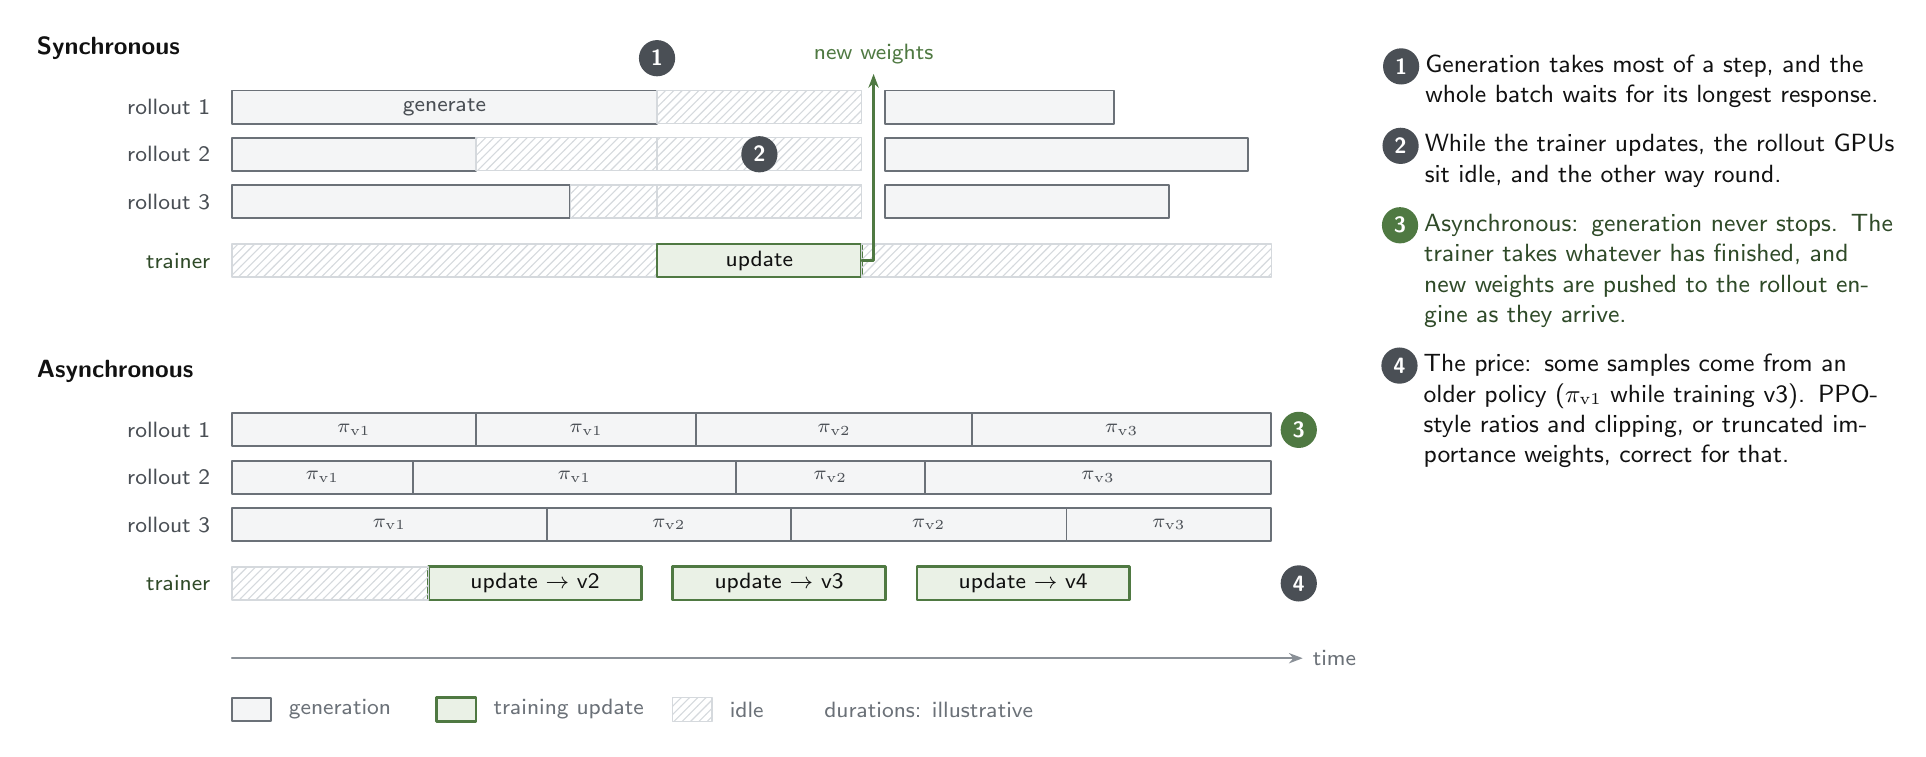
\begin{tikzpicture}[font=\small,
    gen/.style={draw=grey500, line width=0.7pt, fill=grey100},
    upd/.style={draw=fern, line width=1pt, fill=ferntint},
    idle/.style={draw=grey300, line width=0.5pt, pattern=north east lines, pattern color=grey300},
    lane/.style={font=\footnotesize, text=grey700, anchor=east},
    ver/.style={font=\scriptsize, text=grey700},
    ptitle/.style={font=\small\bfseries, anchor=west}]
  \def\h{0.42}
  % ===================== synchronous =====================
  \node[ptitle] at (-2.6,0.75) {Synchronous};
  \foreach \lab/\y in {rollout 1/0, rollout 2/-0.6, rollout 3/-1.2} \node[lane] at (-0.15,\y) {\lab};
  \node[lane, text=ferndark] at (-0.15,-1.95) {trainer};
  % step 1
  \foreach \y/\len in {0/5.4, -0.6/3.1, -1.2/4.3} {
    \draw[gen] (0,{\y-\h/2}) rectangle (\len,{\y+\h/2});
    \ifdim\len pt<5.4pt \draw[idle] (\len,{\y-\h/2}) rectangle (5.4,{\y+\h/2}); \fi
    \draw[idle] (5.4,{\y-\h/2}) rectangle (8.0,{\y+\h/2});
  }
  \draw[idle] (0,{-1.95-\h/2}) rectangle (5.4,{-1.95+\h/2});
  \draw[upd] (5.4,{-1.95-\h/2}) rectangle (8.0,{-1.95+\h/2}) node[midway, font=\footnotesize] {update};
  % step 2 (starts after the weight sync)
  \foreach \y/\len in {0/2.9, -0.6/4.6, -1.2/3.6} \draw[gen] (8.3,{\y-\h/2}) rectangle ({8.3+\len},{\y+\h/2});
  \draw[idle] (8.0,{-1.95-\h/2}) rectangle (13.2,{-1.95+\h/2});
  \node[font=\footnotesize, text=grey700] at (2.7,0) {generate};
  \draw[flowa] (8.0,-1.95) -- (8.15,-1.95) -- (8.15,0.42) node[above, accentnote] {new weights};
  \mk{(5.4,0.62)}{1}; \mk{(6.7,-0.6)}{2};
  % ===================== asynchronous =====================
  \begin{scope}[yshift=-4.1cm]
  \node[ptitle] at (-2.6,0.75) {Asynchronous};
  \foreach \lab/\y in {rollout 1/0, rollout 2/-0.6, rollout 3/-1.2} \node[lane] at (-0.15,\y) {\lab};
  \node[lane, text=ferndark] at (-0.15,-1.95) {trainer};
  % rollouts never stop; the label is the policy version that wrote the sample
  \foreach \y/\a/\b/\v in {0/0/3.1/v1, 0/3.1/5.9/v1, 0/5.9/9.4/v2, 0/9.4/13.2/v3,
                           -0.6/0/2.3/v1, -0.6/2.3/6.4/v1, -0.6/6.4/8.8/v2, -0.6/8.8/13.2/v3,
                           -1.2/0/4.0/v1, -1.2/4.0/7.1/v2, -1.2/7.1/10.6/v2, -1.2/10.6/13.2/v3}
    \draw[gen] (\a,{\y-\h/2}) rectangle (\b,{\y+\h/2}) node[midway, ver] {$\pi_{\mathrm{\v}}$};
  \draw[upd] (2.5,{-1.95-\h/2}) rectangle (5.2,{-1.95+\h/2}) node[midway, font=\footnotesize] {update $\to$ v2};
  \draw[upd] (5.6,{-1.95-\h/2}) rectangle (8.3,{-1.95+\h/2}) node[midway, font=\footnotesize] {update $\to$ v3};
  \draw[upd] (8.7,{-1.95-\h/2}) rectangle (11.4,{-1.95+\h/2}) node[midway, font=\footnotesize] {update $\to$ v4};
  \draw[idle] (0,{-1.95-\h/2}) rectangle (2.5,{-1.95+\h/2});
  \mka{(13.55,0)}{3}; \mk{(13.55,-1.95)}{4};
  \end{scope}
  % time axis
  \draw[grey400, line width=0.6pt, -{Stealth[length=5pt]}] (0,-7.0) -- (13.6,-7.0) node[right, dims] {time};
  % legend
  \draw[gen] (0,-7.5) rectangle (0.5,-7.8); \node[dims, anchor=west] at (0.6,-7.65) {generation};
  \draw[upd] (2.6,-7.5) rectangle (3.1,-7.8); \node[dims, anchor=west] at (3.2,-7.65) {training update};
  \draw[idle] (5.6,-7.5) rectangle (6.1,-7.8); \node[dims, anchor=west] at (6.2,-7.65) {idle};
  \node[dims, anchor=west] at (7.4,-7.65) {durations: illustrative};
  % notes
  \notesat{(14.6,1.0)}{6.0cm}
  \note{1}{Generation takes most of a step, and the whole batch waits for its longest response.}
  \note{2}{While the trainer updates, the rollout GPUs sit idle, and the other way round.}
  \notea{3}{Asynchronous: generation never stops. The trainer takes whatever has finished, and new weights are pushed to the rollout engine as they arrive.}
  \note{4}{The price: some samples come from an older policy ($\pi_{\mathrm{v1}}$ while training v3). PPO-style ratios and clipping, or truncated importance weights, correct for that.}
\end{tikzpicture}
\end{document}
